\section{Nebulas Rank}
\label{sec:rank}

\subsection{价值尺度总体设计} \label{subsec:value}
当前区块链技术和生态已具有相当规模,但是人们对其认识还处于扁平化阶段,尚不存在一个合理的方式去评估链上实体(例如用户地址)的价值。因此,我们试图在区块链世界提出⼀个普适的价值尺度,通过对链上行为的挖掘利用,将每个实体(用户地址)的重要程度量化为\textbf{Nebulas Rank}的指标形式。\textbf{Nebulas Rank}旨在实现双重目标:
\begin{itemize}
	\item 作为原生的价值尺度,\textbf{Nebulas Rank}可以成为诸多基础场景的核心算法,如共识算法(见\refsec{sec:pod})、开发者激励(见\refsec{sec:dip})和区块链搜索引擎(见\refsec{sec:search}),等等;
	\item \textbf{Nebulas Rank}可以启发人们对区块链的生态现状定义更多样化的价值尺度,同时产生更深层次、差异化和结构化的认识,进而在商业决策和研究活动中有明确的方向;
\end{itemize}
基于上述目标,我们为\textbf{Nebulas Rank}定义了三重价值尺度:
\begin{itemize}
	\item 流动性,即交易的频次和规模,是\textbf{Nebulas Rank}的第⼀个考量维度。本质上来看,⾦融是通过资本流动推动社会资源的有效配置、推动经济发展的社会活动。区块链构建了⼀个价值⽹络,更多的交易数量、更⼤的交易规模产⽣更⾼的流动性,更⾼的流动性⼜进⼀步提升了交易数量、交易规模,从⽽进⼀步强化了它们的价值,形成了⼀个完整的正向反馈机制。 
	\item 传播性,即资产流动的⼴度和深度,是\textbf{Nebulas Rank}的第⼆个考量维度。在社交网络中的传播性,即信息的传播速度、⼴度和深度,是⽹络质量和⽤户增长的关键指标。我们在区块链世界将会看到同样的模式,强⼤传播性意味着资产流动的⼴度和深度,会提⾼区块链世界的资产质量,提升资产规模。
	\item 互操作性是\textbf{Nebulas Rank}的第三个考量维度。在互联⽹的早期,我们只有简单的⽹站,孤⽴的信息。现在,⽹络上的各种平台信息开始相互调⽤,数据孤岛逐渐被打破。这⼀趋势可以被理解为识别更⾼维度信息的过程。我们认为区块链世界也会遵循同样的发展规律,但其过程速度会更快。⽤户的资产、智能合约和DApp之间的信息会越来越丰富,⾼维信息间的互操作会越来越频繁,因此更好的互操作性将会变得越来越重要。 
\end{itemize}

我们选择使用链上的交易记录作为\textbf{Nebulas Rank}算法的数据来源。因为相比于现实世界,区块链世界的『行踪』更为清晰和可信:链上的交易数据忠实地记录了用户之间的每笔转账、以及每次对『智能合约』的调用情况。然而根据交易数据设计算法并非易事。因为相比于现实世界,区块链世界的交易具有天然的匿名性,同时数据量规模更为庞大。因此我们试图为\textbf{Nebulas Rank}刻画如下的性质:
\begin{itemize}
	\item 可信。实体如果要提高自己的价值,必须付出一定的成本,这样可以确保算法的结果能够甄选出真正具有较高价值的用户。一方面,在共识算法和开发者激励等场景下,可信的结果鼓励用户诚实地贡献以实现正向反馈,另一方面,可信的结果提供了有意义的用户分层结果,能提供更好的决策基础。
	\item 可计算。作为基础字段,\textbf{Nebulas Rank}的结果应该以最快最直接的方式提供,因此其实现需要较低的计算复杂度;
	\item 可复现。由于共识算法和开发者激励等场景的需要,\textbf{Nebulas Rank}需要保证在所有客户端的计算结果完全一致。
\end{itemize}

接下来我们设计\textbf{Nebulas Rank}的基本框架。首先,我们用图的形式表现交易记录。在交易图的基本定义中,每个节点代表一个实体,每条边代表实体之间的转账行为\cite{Tschorsch2015}。交易图表现了转账行为导致资产流动的性质,有助于表示上述价值尺度中流动性和传播性的概念。同时,图的形式也能方便刻画合约之间的互操作性。得到图之后便可以用复杂网络的中心性测度来对重要网络节点进行排序,对\textbf{Nebulas Rank}的情景,我们采用LeaderRank\cite{Chen2013}\cite{Li2014},并取得比PageRank和NEM\cite{nem}的NCDAwareRank更好的排序效果。

\subsection{交易图} \label{subsec:txg}
本小节介绍如何从交易数据构造交易图。

首先,取近期$T$个区块内个人用户对个人用户的有效转账记录,记为$T_{xs}$:
\begin{align}
T_{xs} = \{(s,t,\tau, a)| \tau = \#CurrentBlock-T \dots \#CurrentBlock \land a > 0 \}
\end{align}
,$s$、$t$和$a$分别是转出地址、转入地址和转账金额。

然后基于$T_{xs}$,构造有向加权简单图$G=(V, E, W)$,其中,节点集合、边集合和边权分别表示为$V$, $E$和$W$。另外,记$N = |V|$,$M = |E|$。 简便起见,所有节点都以一个$1$到$N$之间的整数代表。

每个节点都代表一个账户的地址,每条边代表两个用户之间的转账强度。规定所有边有向,并按如下公式合并对应交易的最高$K$个金额作为权值$w_e$:
\begin{align}\label{formula:edgeweight}
w_e = \sum_{i=1}^K a_i, s.t. a_i \in \{a|(s,t,\tau,a) \in T_{xs} \} \land a_1 \geq a_2 \dots
\end{align}

接着,对每个节点,根据其在过去$T$个区块的转入转出记录,计算它的『币龄』,记作$C_v$;根据转入转出的金额总量,根据\reffig{fig:encouragement}所示的『鼓励函数』计算出每个节点鼓励值$E_v$\footnote{鼓励函数可以表示为两个正态分布的线性加和形式,在转出金额为零时以及转出金额少于转入金额的某点取得最大值}。最后使用目标节点的$C_v$和$E_V$对边权进行衰减。

\begin{figure}
\centering
	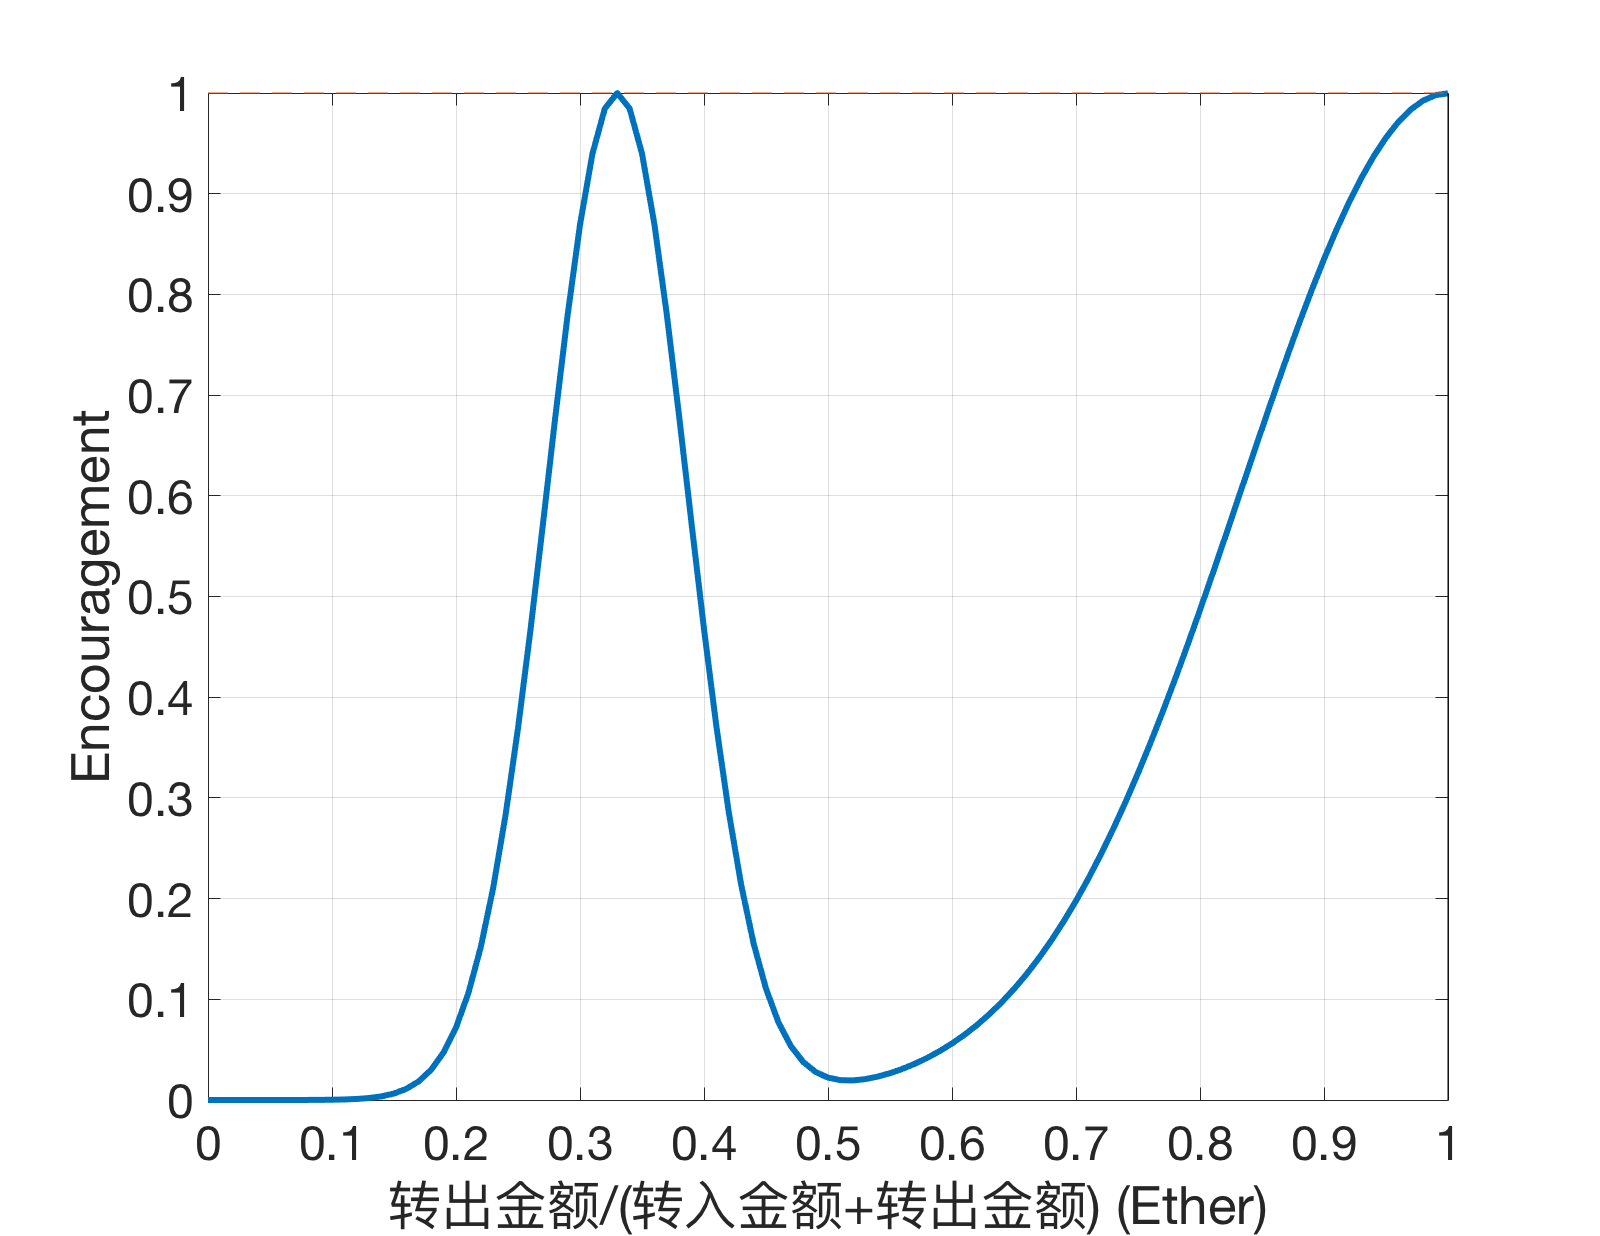
\includegraphics[width=0.55\textwidth]{figs/encouragement.png}
	\caption{鼓励函数}\label{fig:encouragement}
\end{figure}


最后,取整个交易图的最大弱连通分支,将分支之外的节点删除。

上述构造交易图的方式有助于实现\refsec{subsec:value}定义的『可信』性质,具体效果见\refsec{subsec:robust}的讨论。

我们收集了Ethereum主链从\#3629091(约2017年5月1日)到\#3800775(约2017年5月31日)共$171,684$个区块交易数据,按照本小节介绍的方式构造了交易图($T=171,684$ , $K=2$),可视化结果如\reffig{fig:wgc}所示。

\begin{figure}
	\centering
	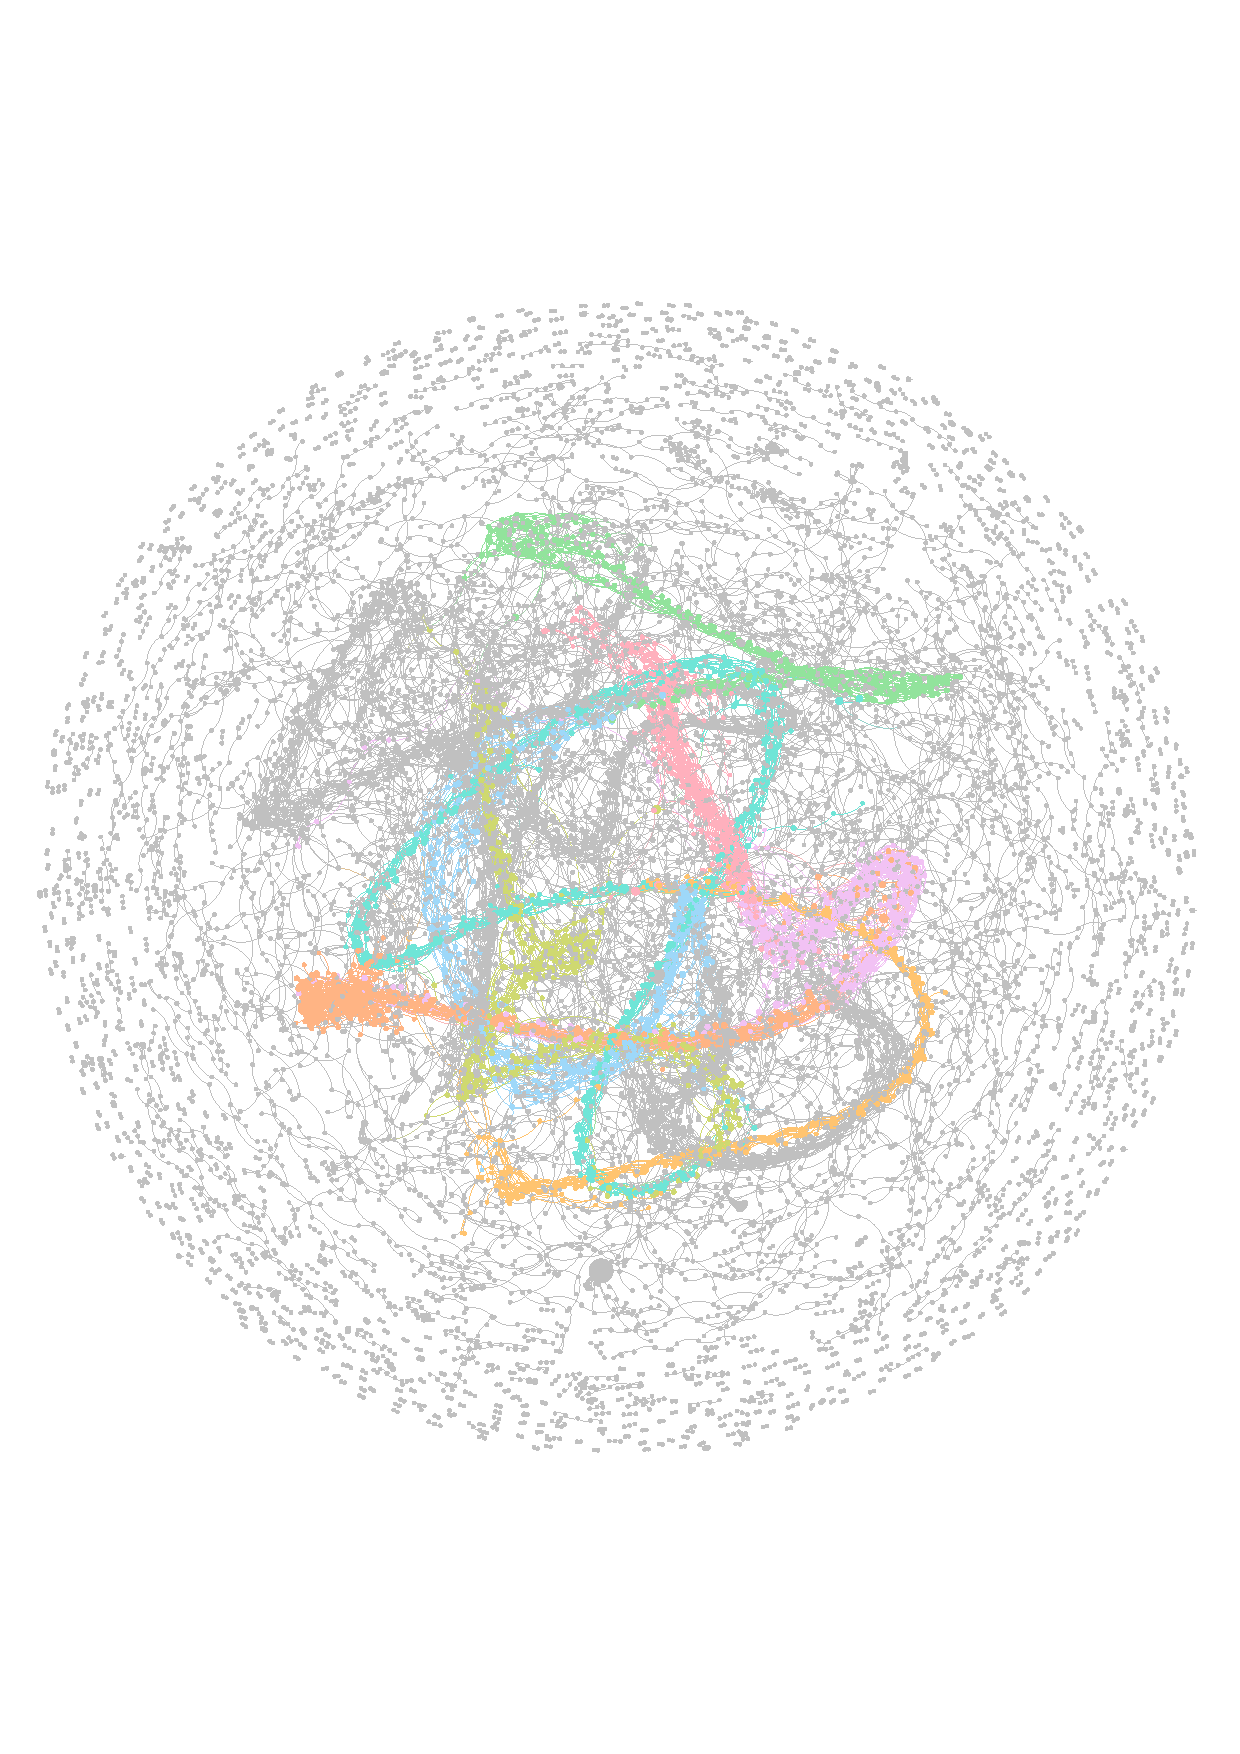
\includegraphics[width=0.85\textwidth]{figs/wgc.pdf}
	\caption{交易图可视化结果}\label{fig:wgc}
\end{figure}


\subsection{排序算法} \label{subsec:leaderrank}
本小节介绍如何在构造的交易图中进行节点重要性排序。

我们采用LeaderRank\cite{Chen2013}\cite{Li2014}作为核心算法。首先在交易图中添加Ground节点,记为$\mathcal{G}$,编号$N+1$。然后我们建立Ground节点和其他每个节点的双向链接,并按照接下来的方式赋予链接权值:
\begin{align}\label{formula:weight1}
	\forall v \in V, w_{(v, \mathcal{G})} = \alpha A_v
\end{align}
\begin{align}\label{formula:weight2}
\forall v \in V,  w_{(\mathcal{G}, v)} = \beta B_v
\end{align}
其中:
\begin{align}
	\forall v \in V, A_v = \{ \sum_{(u,v)\in E} w_{(u,v)} - \sum_{(v,u) \in E} w_{(v, u)}, 0 \} + \lambda C
\end{align}
\begin{align} \label{formula:b}
\forall v \in V,  B_v =  \sum_{(u,v) \in E} w_{(u,v)} + \mu C
\end{align}
\begin{align}
	C = median\{w_e| e \in E\}
\end{align}

$\alpha, \beta, \mu, \lambda$为参数。上述赋权方式可以理解为,入度更大的节点接收了更多来自Ground节点的入边权值,『净流入』,即入度减出度,更大的节点向Ground节点输出了更强的链接。

LeaderRank的计算过程和PageRank基本相同,可以理解为求马可夫链的稳定状态。所不同的是,添加了Ground节点之后,不再需要考虑PageRank的damping factor\cite{Brin2010}\cite{page1999pagerank}。即按(\ref{formula:matrix})构造矩阵$H$后,进行如(\ref{formula:iteration})所示的迭代(初始值设置见(\ref{formula:init})),直至收敛为止,最后去掉Ground节点的评分即为交易图各点重要程度得分。

\begin{align} \label{formula:iteration}
	P^{t+1} = H \times R^{t}; P^1=[\frac{1}{N}, \frac{1}{N}, \dots, \frac{1}{N}, 0]^T
\end{align}
\begin{align} \label{formula:matrix}
	h_{ij} = \frac{w_{(j,i)}}{\sum_k w_{(j,k)}}
\end{align}
\begin{align} \label{formula:init}
\forall v \in V, P^*_v \leftarrow P^*_v + \frac{P^*_{\mathcal{G}}}{N}
\end{align}


我们认为,LeaderRank可以较好地满足\refsec{subsec:value}定义的价值尺度和算法性质:
\begin{itemize}
	\item LeaderRank可以理解为在资金流动网络动态平衡状态下通过每点的流量,这契合了\textbf{Nebulas Rank}的『流动性』、『传播性』和『互操作性』等尺度;
	\item (\ref{formula:weight2})和(\ref{formula:b})所定义的赋权机制可以加大攻击难度(见\refsec{subsec:robust}的讨论),更好地满足『可信』性质;
	\item LeaderRank的计算可以用迭代方式完成,由于网络的稀疏性(见\refsec{subsec:txg}的结果),矩阵运算复杂度不高,能够满足『可计算』和『可复现』的性质。
\end{itemize}


\subsection{抵抗操纵}\label{subsec:robust}

可信性,即抵抗操纵的能力,是\textbf{Nebulas Rank}最重要同时也是最具挑战的指标。部分恶意操纵的手段有以下几种:
\begin{itemize}
	\item 环形转账,攻击者沿环形拓扑,让同一笔资金不断流过对应的边,以提高边权;
	\item 频繁同权威交易所账户交易,多次在交易所账户中取入取出同一笔资金,在网络结构中获得更好的位置;
	\item 向其他任意账户转钱,提高出度,并且提高资金流出的传播性;
	\item 控制多个账户形成独立分支,伪造中心节点;
\end{itemize}

\textbf{Nebulas Rank}通过以下几个机制,可以弱化操纵效果:
\begin{itemize}
	\item 由于设置了$T$个区块的滑动时间窗,攻击者无法在短期内迅速提高自己的排名;
	\item 因为边权由最高的几次交易金额决定,在一个环状拓扑内的多次转账不能无限提高各边权值,同时,从\refsec{subsec:txg}采集的数据看,有$91\%$的双方只进行了一或两次交易,因此$K$取$2$可以最大限度保留边的强度信息,同时抵抗环形转账攻击;
	\item 为了获得更高『币龄』,用户需要让资金在自己的账户内『停留』一段时间,进而拖慢攻击者的交易速度;
	\item 为了获得最大的『鼓励值』,如\reffig{fig:encouragement}所示,账户需要在当前周期内储蓄全部收入,或者只转出少于收入一半的金额,因此伪造资金流动时,攻击者的本金会因各个账户的储蓄效应而迅速衰减;
	\item 由于取了最大弱联通分支,伪造的独立分支会被视为噪声而过滤清除。从\refsec{subsec:txg}采集的数据看,交易图有$453,285$个节点,$970,577$条边,有$1,169$个弱分支,其中最大弱分支有$449,746$个节点,占全体节点的$99.2\%$,次大弱分支有$133$个节点,仅占全体节点的$0.03\%$,因此取最大联通分支可以最大限度保留网络正常成分并且过滤噪声数据;
	\item 相对于PageRank和NCDawareRank\cite{Nikolakopoulos2013}等网页排序算法,(\ref{formula:weight2})和(\ref{formula:b})所定义的赋权机制对低入度的节点评分偏向『保守』,即低入度的节点获得来自Ground节点的链接更弱。在区块链交易图中,低收入节点更容易被伪造,因此使用\textbf{Nebulas Rank}的方法可以提升操纵难度;
\end{itemize}

接下来,基于2017年5月份Ethereum的交易图(见\refsec{subsec:txg}),我们展示一系列结论。

首先对比交易金额和\textbf{Nebulas Rank}的关系。由于区块链交易可以理解为『资金交换』类型的网络流,根据\textcite{Borgatti2005}的研究工作,节点的度,即邻接边权值之和,是适用于此类网络的一个合适的中心性测度。以每个节点为中心思考,度,即交易金额(转入转出金额的和),是节点一跳局部信息的体现,直接反映了对应地址的历史资金流量,因此应该作为衡量排序算法的基准。交易金额与\textbf{Nebulas Rank}的关系如\reffig{fig:nrio}所示:没有节点能够具有较少的交易金额却获得了较高的权值,这可以大致印证\textbf{Nebulas Rank}的可信性;交易金额与PageRank和NCDawareRank的关系如\reffig{fig:prio}和\reffig{fig:ncdio}所示:有部分节点权值较高却只有少量交易额,这表明在实际网络中,攻击者可以寻找适当的拓扑位置,以较少的本金获得靠前的排名;

\begin{figure}
	\centering
	%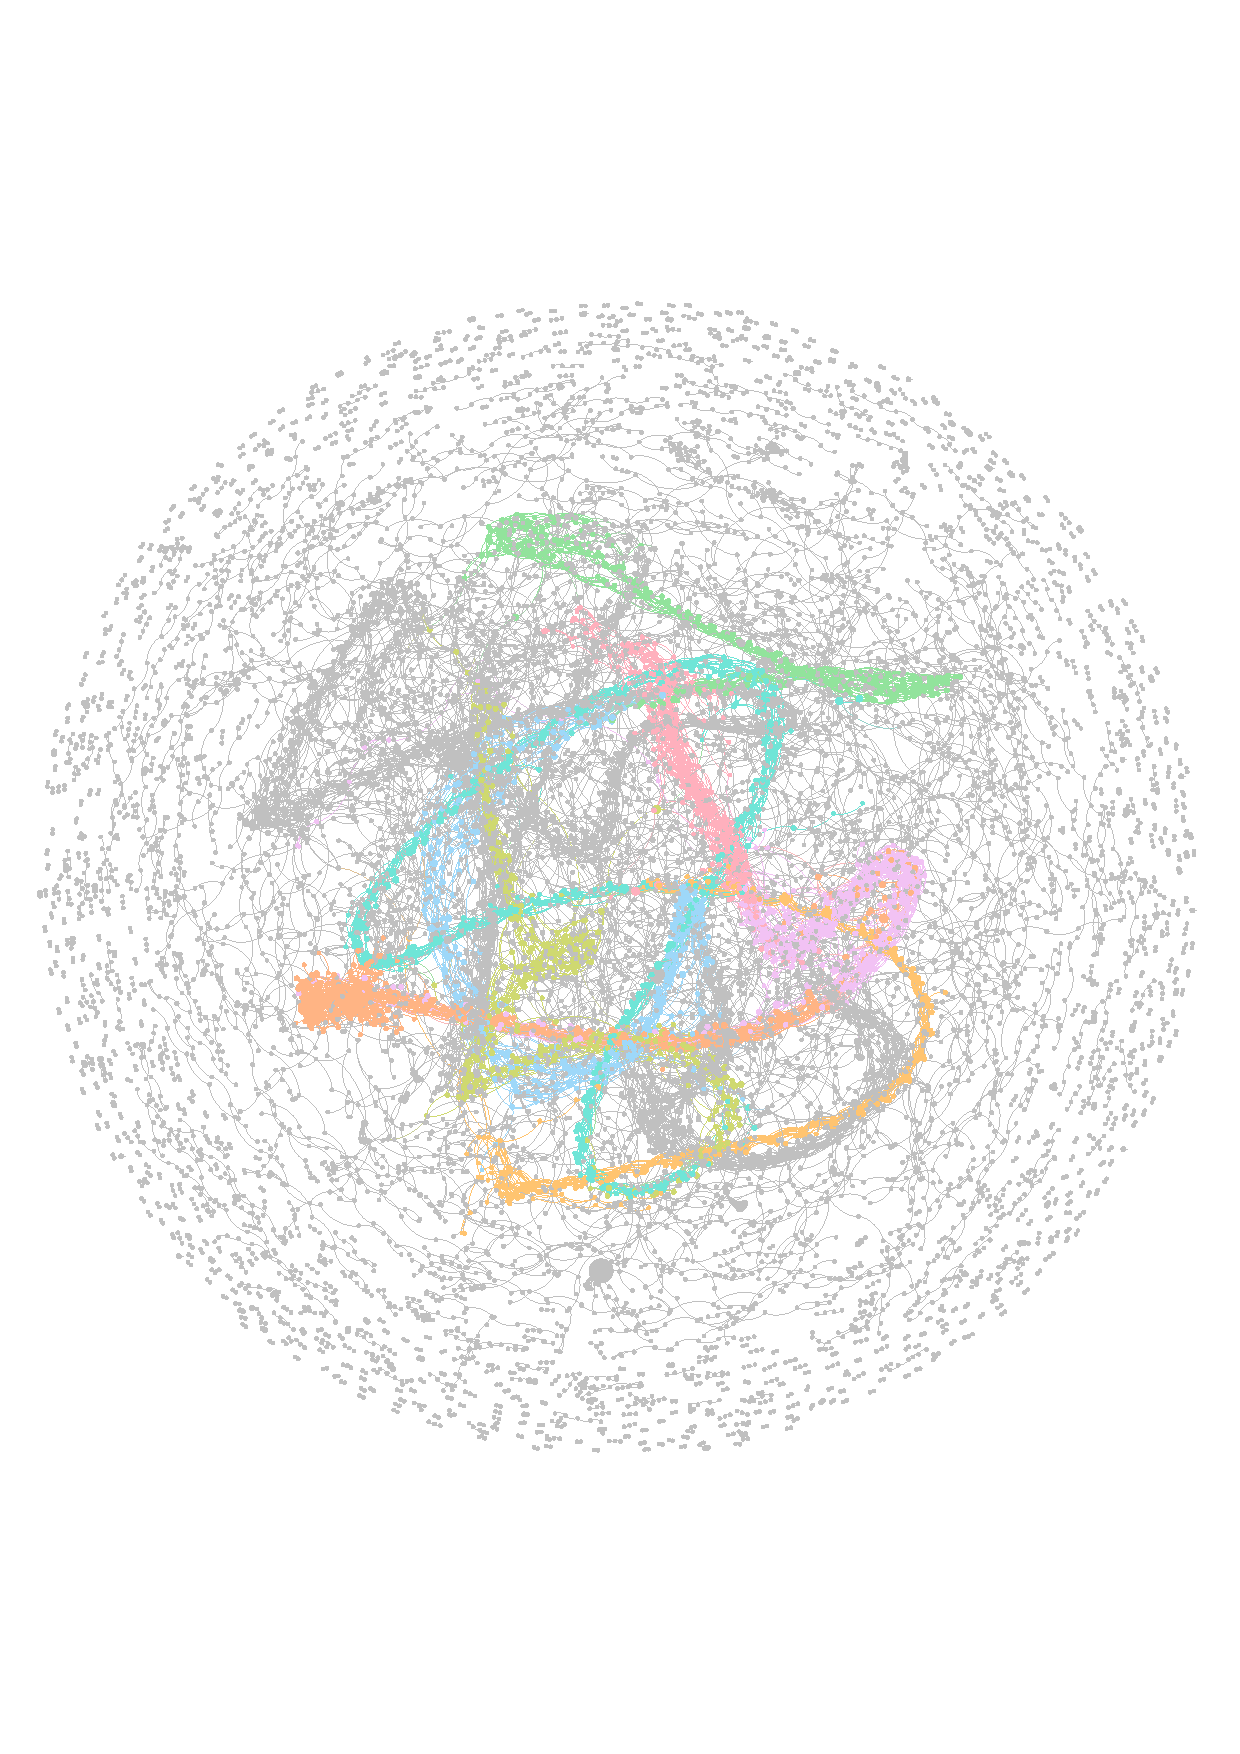
\includegraphics[width=0.85\textwidth]{figs/wgc.pdf}
	\caption{Nebulas Rank v.s. 交易金额}\label{fig:nrio}
	\caption*{note}
\end{figure}

\begin{figure}
	\centering
	%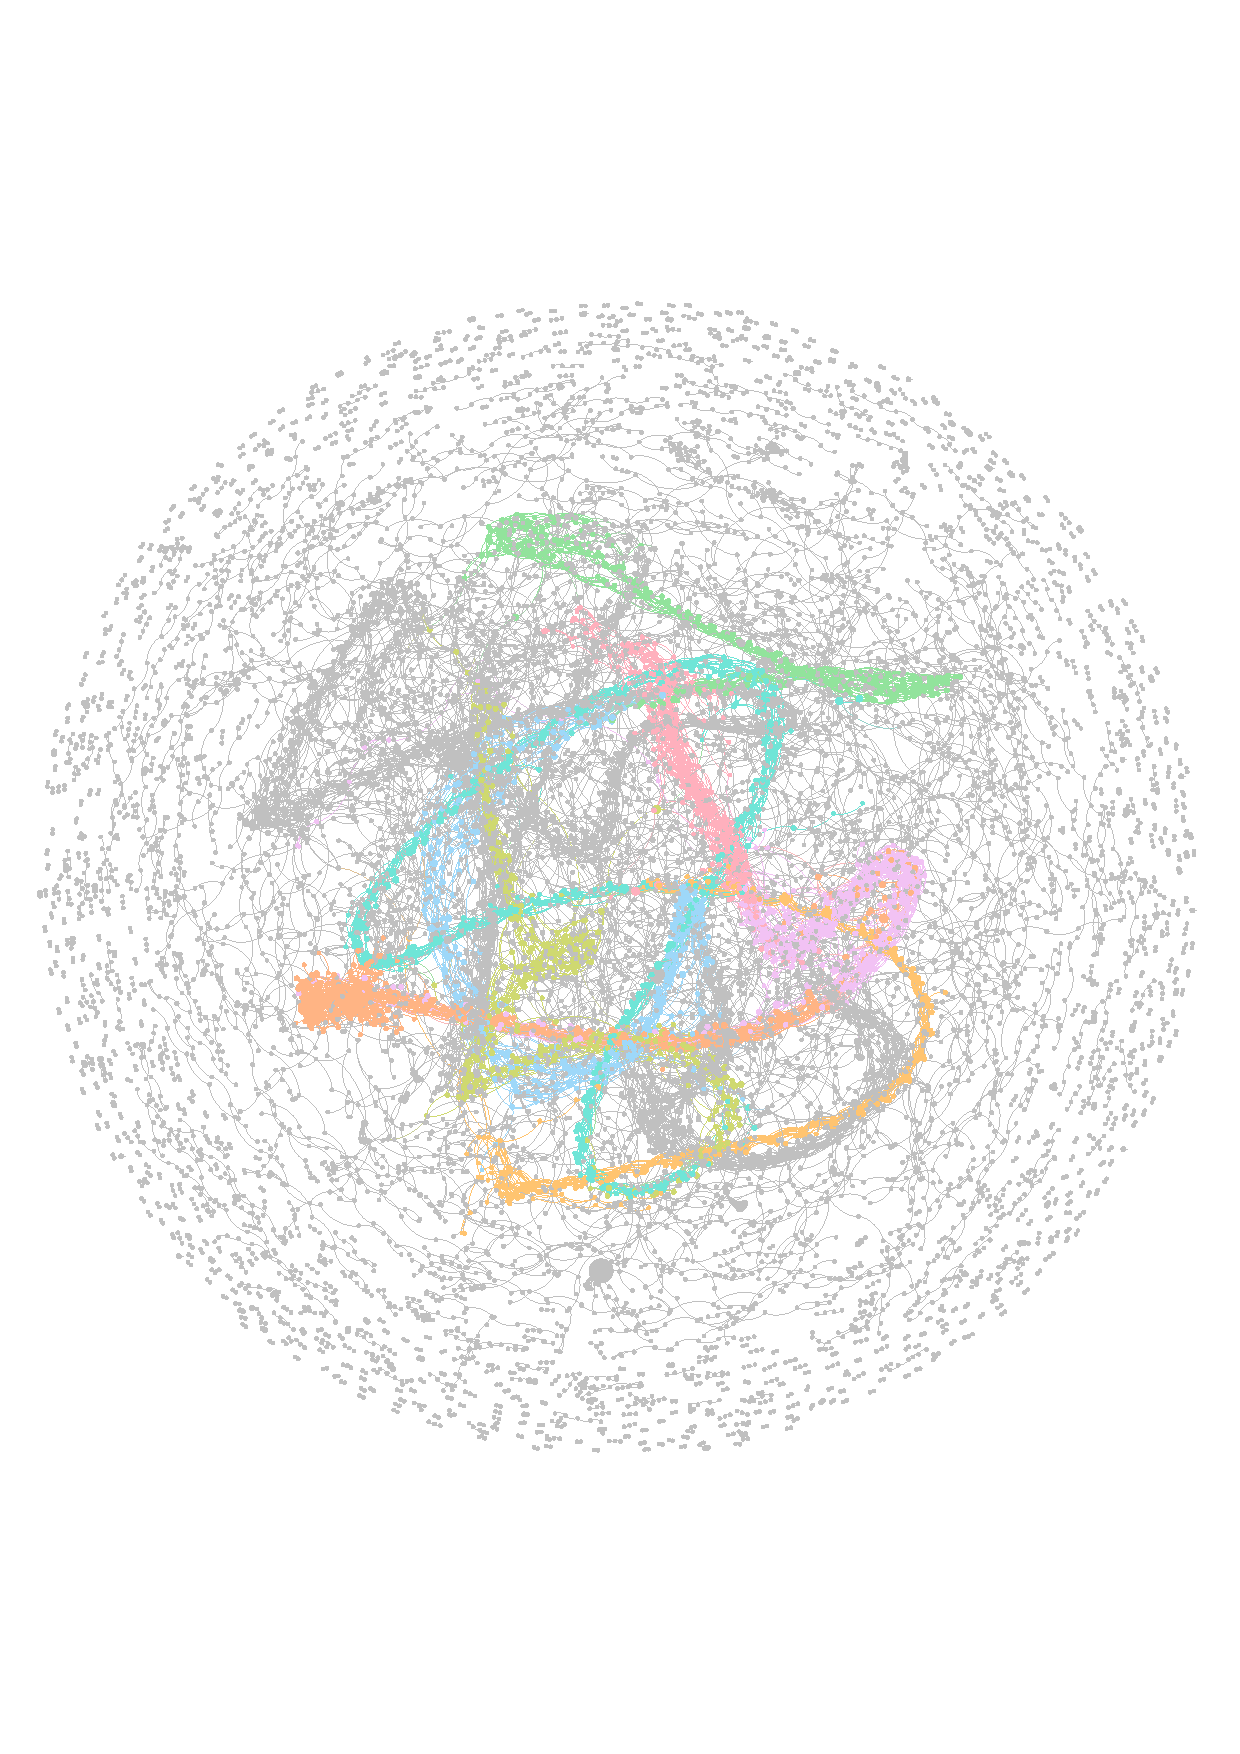
\includegraphics[width=0.85\textwidth]{figs/wgc.pdf}
	\caption{PageRank v.s. 交易金额}\label{fig:prio}
	\caption*{note}
\end{figure}

\begin{figure}
	\centering
	%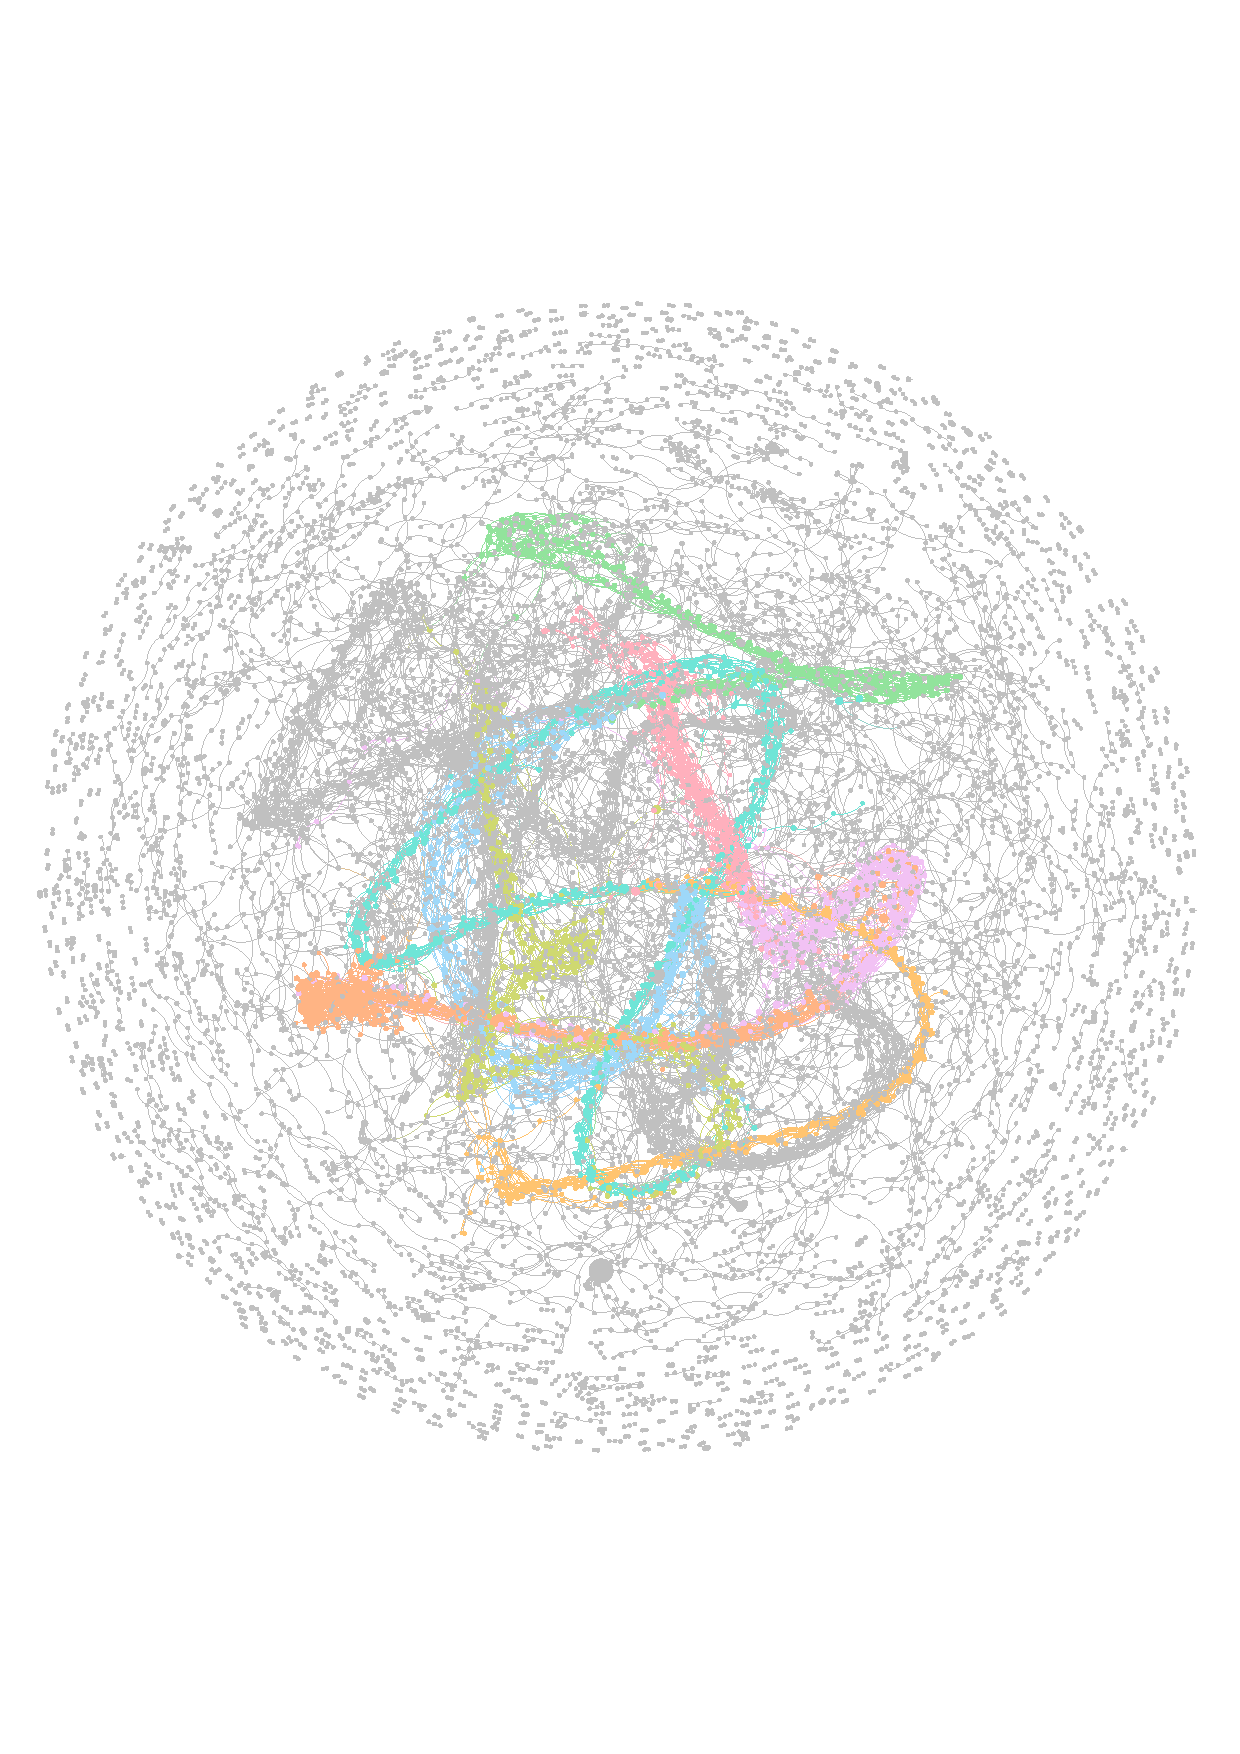
\includegraphics[width=0.85\textwidth]{figs/wgc.pdf}
	\caption{NCDawareRank Rank v.s. 交易金额}\label{fig:ncdio}
	\caption*{note}
\end{figure}

接着,我们列出各算法排名前$10$名的地址,如表\ref{}所示。。。。。


最后,我们仿真一类特定的攻击,攻击者选定某权威交易所节点,在排名计算周期内创造$X$次环形交易,每次交易时,攻击者先经由某新建地址向交易所节点转入$Y$Ether,之后经另一新建节点从交易所节点取出$Y$Ether,攻击方式示意图如\reffig{fig:loop}所示。测试选择的交易所为Poloniex Wallet(0x32be343b94f860124dc4fee278fdcbd38c102d88),结果如\reffig{fig:antiManipulation}所示,。。。。

\begin{figure}
	\centering
	%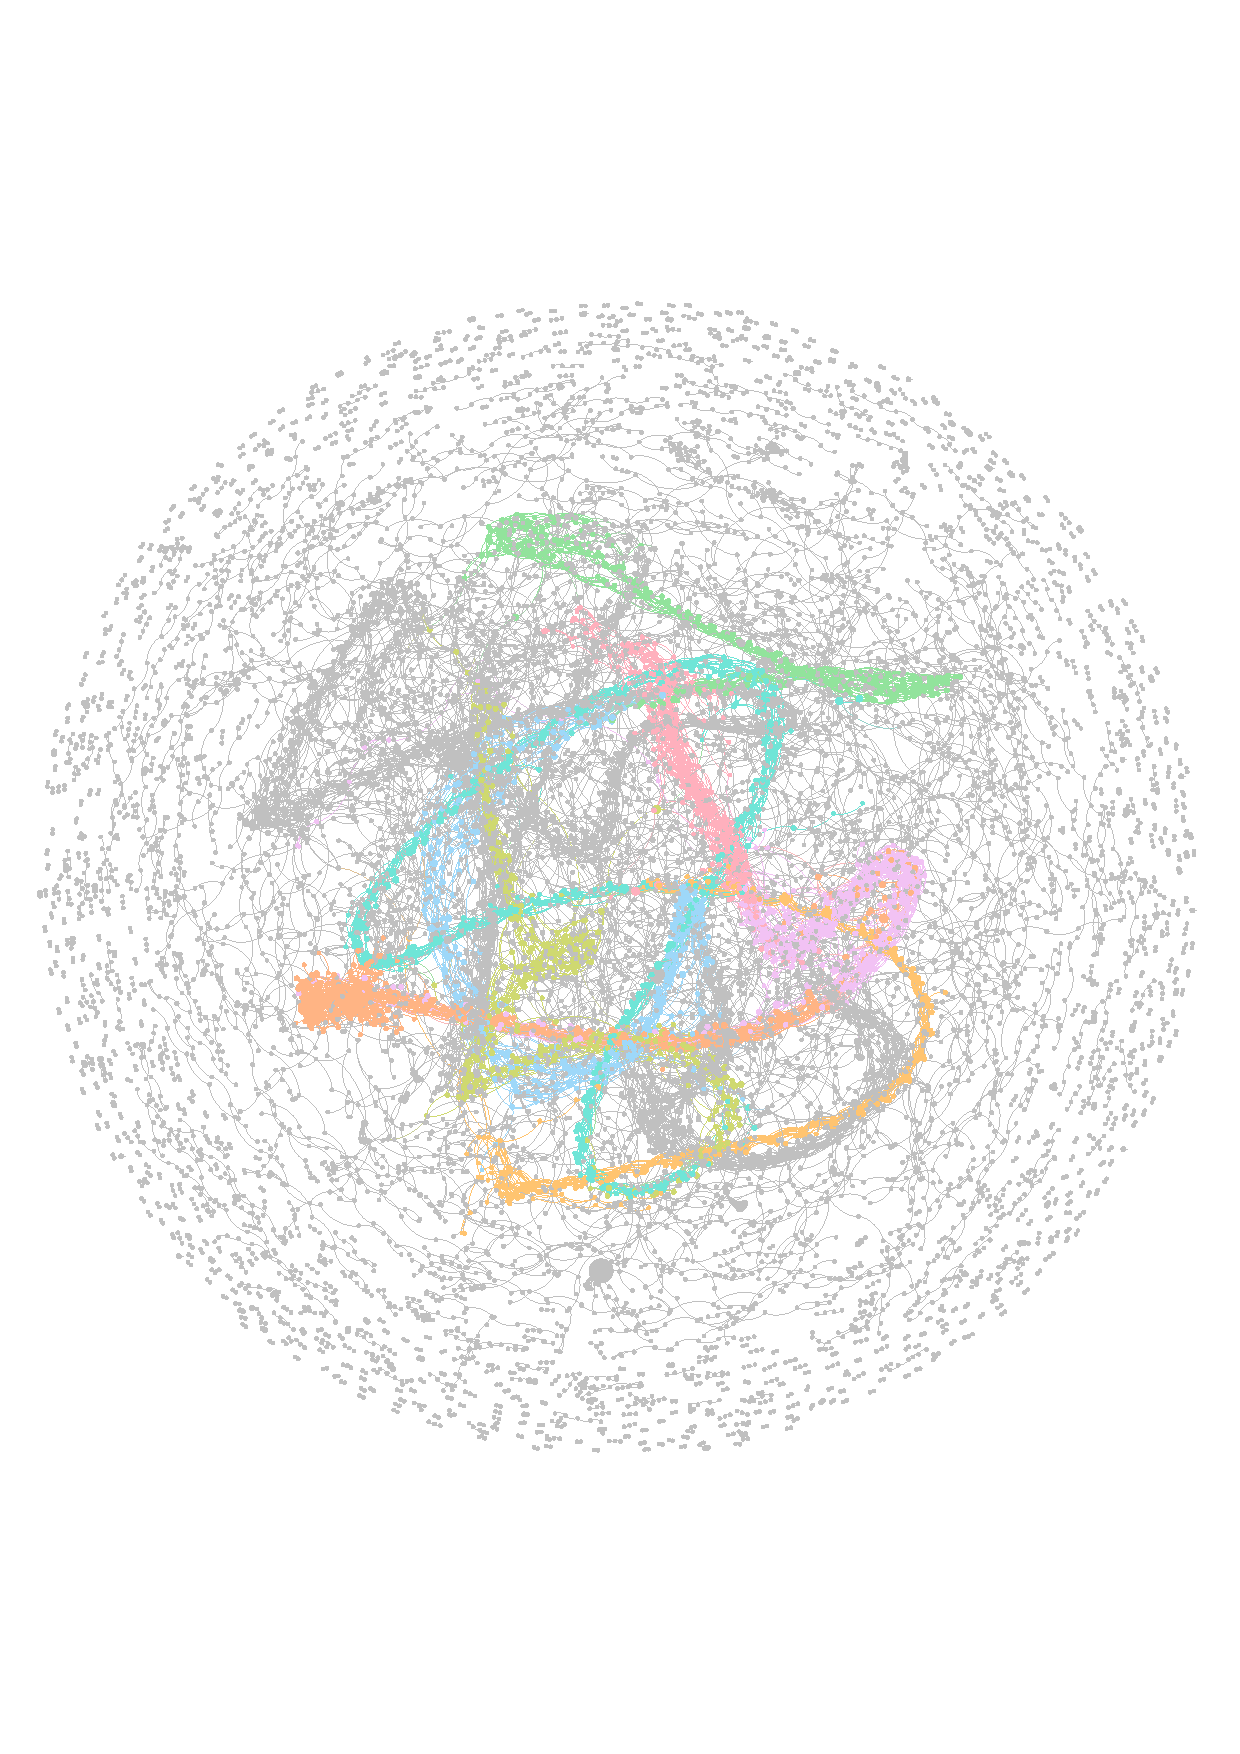
\includegraphics[width=0.85\textwidth]{figs/wgc.pdf}
	\caption{将交易所纳入环形交易的攻击示意图}\label{fig:loop}
	\caption*{note}
\end{figure}

\begin{figure}
	\centering
	%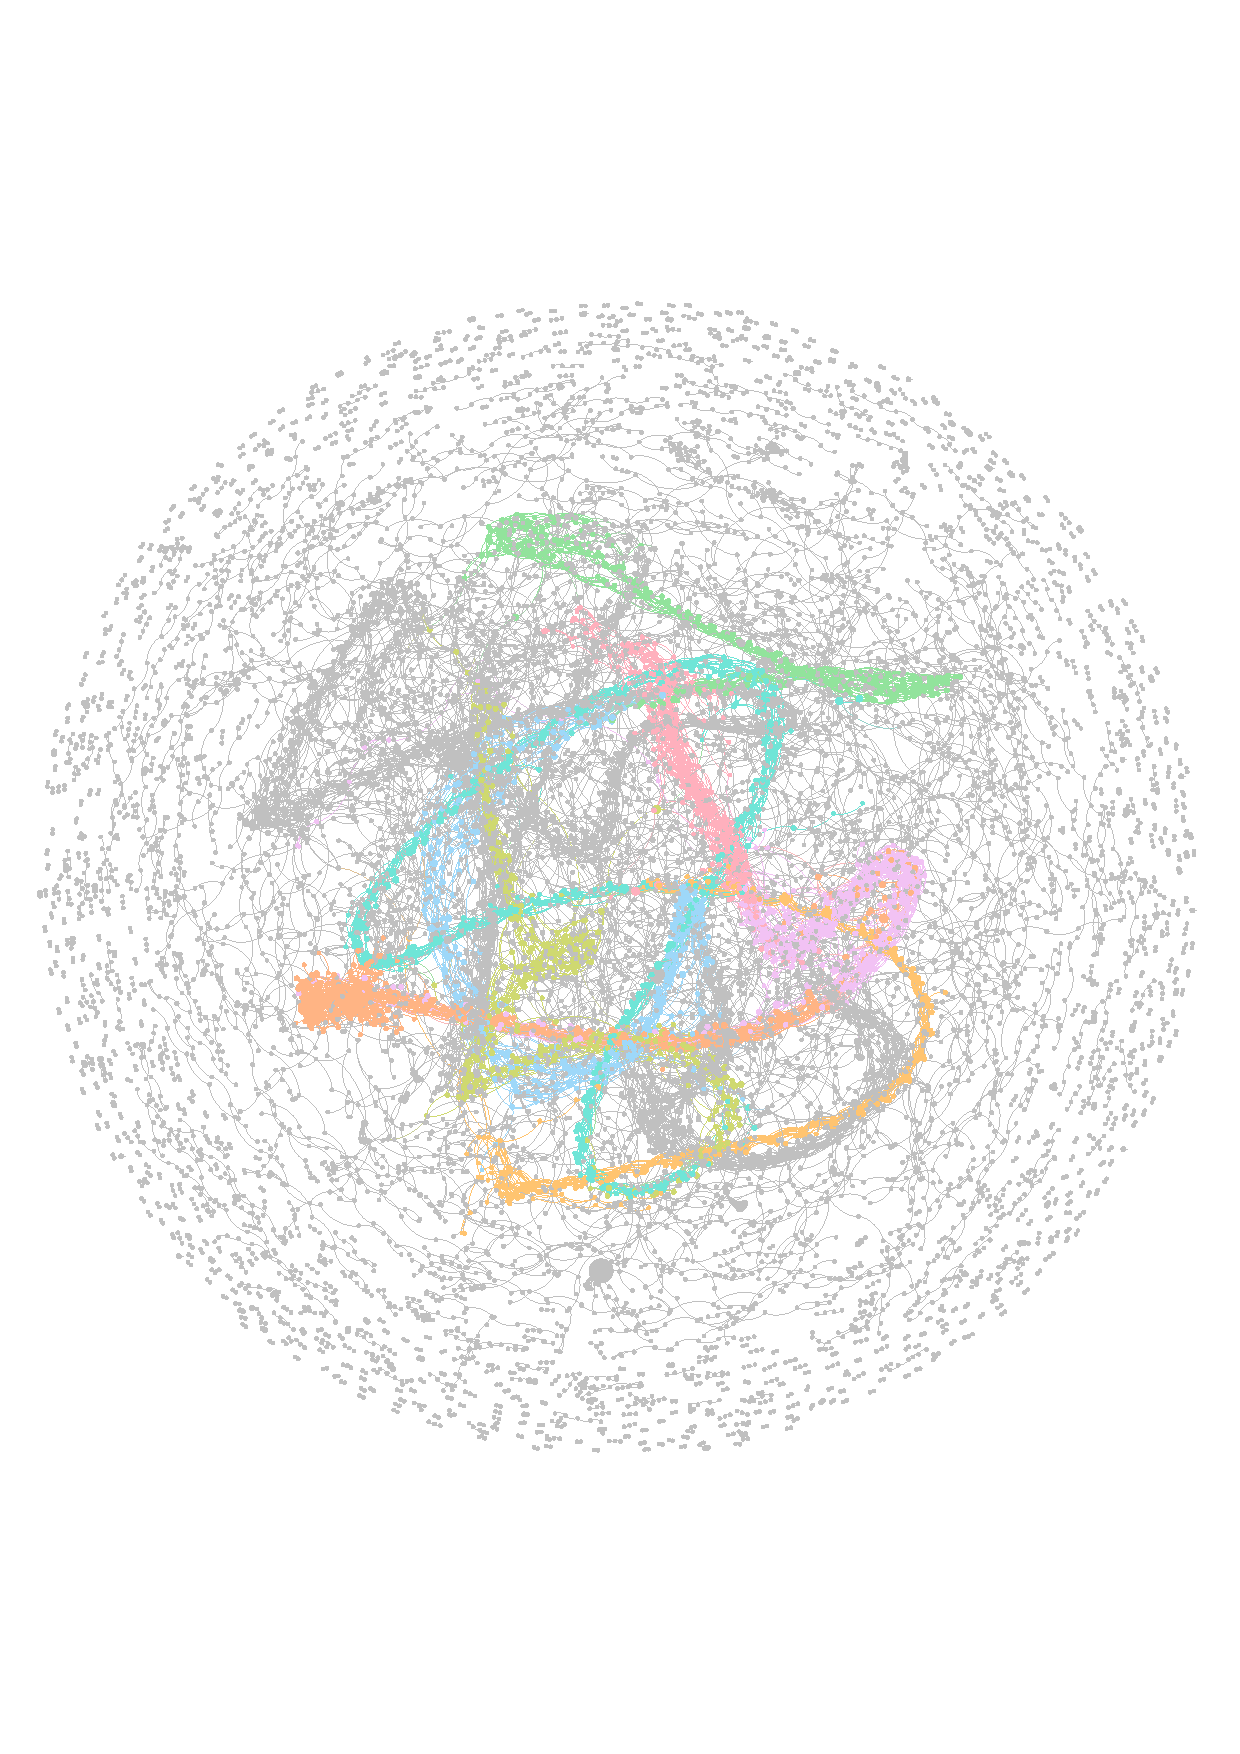
\includegraphics[width=0.85\textwidth]{figs/wgc.pdf}
	\caption{抗操纵测试结果}\label{fig:antiManipulation}
	\caption*{\footnotesize{NR:交易图如\refsec{}所述,排序算法按照\refsec{}所述;\\PR$^*$:交易图如\refsec{}所述,PageRank排序算法;\\ NCD$^*$:交易图如\refsec{}所述,NCDawareRank排序算法;\\ NCD$^{\#}$:交易图如\cite{nem}所述,NCDawareRank排序算法;\\ PR$^{\#}$:交易图如\cite{nem}所述,PageRank排序算法 \\ PageRank的damping factor为0.15;NCDawareRank使用pscan\cite{}社群划分算法,$\eta=$, $\mu=$}}
\end{figure}

\subsection{相关工作}
中心性,作为最核心的节点排序指标,是过去几十年网络科学领域研究最多的一个概念\cite{newman2010networks}。丰富的文献引入了大量中心性测度,包括度中心性\cite{freeman1979set}, 特征值中心性\cite{bonacich1972factoring}, Katz中心性\cite{katz1953new}, 接近度中心性\cite{sabidussi1966centrality}, 介数中心性\cite{freeman1977set}\cite{freeman1978centrality}\cite{freeman1991centrality}\cite{noh2004random}\cite{newman2005measure}, PageRank\cite{Brin2010}, HITS\cite{kleinberg1999authoritative}, SALSA\cite{Science2001}, 等等。此外还有许多工作试图用统一的框架来对中心性测度作出清晰的分类和综述\cite{Borgatti2005}\cite{Borgatti2006}\cite{Lu2016}。在设计\textbf{Nebulas Rank}时,需要首先考察交易图的性质,然后再选用合适的中心性。\textcite{Borgatti2005}工作中提到的资金交换网络和区块链交易图最为相近,但是提到的相关算法,如流中心性\cite{freeman1991centrality} 和随机游走中心性(又称电流中心性)\cite{newman2005measure},复杂度过高,在区块链交易图的规模上不符合\textbf{Nebulas Rank}的『可计算』性质。

自从比特币\cite{Nakamoto2008}系统在2009年发布以来,研究者们对比特币交易图做了一些试验性和统计上的分析\cite{Ron}\cite{Haslhofer}\cite{NielKondor2014}\cite{Baumann2014}, 同时试图使用交易图的结构来讨论比特币的匿名性问题\cite{Meiklejohn2013}\cite{Ober2013}\cite{pham2016anomaly}\cite{Fleder2015}\cite{Ferrin2015}。 在其他加密货币出现并流行之后,交易图分析拓展到了其他的区块链系统\cite{Chang2017}\cite{Anderson2016}。 \textbf{Nebulas Rank}采用的交易图概念和这些研究中的大致相同,即\textcite{Tschorsch2015}所总结的『实体图』。即每个用户实体被映射为一个节点。而每条有向边则代表两个用户之间的交易强度。事实上,早在如比特币一样的区块链系统发明之前,学者们就尝试对银行和国际交易的金融网络进行研究\cite{propper2008towards}\cite{Boss2004}\cite{Serrano2007}\cite{Bech2008}\cite{Fagiolo2009}\cite{Morten2006}\cite{Boss2004a}\cite{Krempel2002}\cite{Serrano2003}。 和区块链交易图相比,这些早期研究的网络还包含了额外的借贷活动。并且这些网络的规模非常小。总之,现有研究几乎没有专门针对大规模区块链交易图提出排序方法。

和\textbf{Nebulas Rank}最相关的工作是 NEM\cite{nem}的Proof-of-Importance机制,它采用了 NCDawareRank\cite{Nikolakopoulos2013}作为排序算法。 NCDawareRank\cite{Nikolakopoulos2013}利用了网络拓扑的社群效应。Proof-of-Importance使用SCAN\cite{xu2007scan}\cite{shiokawa2015scan}\cite{chang2017mathsf}作为社群聚类算法。虽然社区结构在交易网络的确存在并且可以帮助应对欺诈节点,却无法保证同一个实体对应节点一定可以映射到相同社群,因此利用社区划分的结果会提供一定的可操纵空间。此外\textcite{Fleder2015}使用PageRank来帮助发现感兴趣的比特币地址并分析它们的活动,但他们的工作仍然将人工主观分析作为主要方法,PageRank只起到辅助作用,这也和\textbf{Nebulas Rank}的目标不符。

我们采用的算法时LeaderRank\cite{Chen2013}\cite{Li2014}。 它是PageRank的一种拓展形式。\todo{在PageRank中,开始每个节点都拥有一单位的rank值。之后的每轮迭代中,每个节点将自己的rank值平均分配给每个直接邻居。此外,PageRank存在damping因子:每个节点都以一定概率将自己的rank值均匀分配给网络中的全部节点。\textcite{Chen2013}对damping因子提出了一种简单但有效的改进。然后\textcite{Li2014}将LeaderRank拓展至加权场景并进一步提升了效果。加权的LeaderRank算法在网络中加入了一个额外的ground节点,并在每个节点与Ground节点之间建立了双向链接。每条指向Ground节点的边权都相同,而每条由Ground节点指出的边权都正相关于目标节点的入边总额。LeaderRank比PageRank可以更好地抵抗操纵和噪声数据\cite{Chen2013}\cite{Li2014}\cite{Lu2016}。 在计算过程上,LeaderRank可以看作是加了额外节点但没有damping因子的PageRank。因此它也很容易实现同时适应超大规模网络。}
 